\chapter{Background}
\label{sec:background}

% Background on design of DynamoRIO, all relevant considerations.

%%%%%%%%%%%%%%%%%%%%%%%%%%%%%%%%%%%%%%%%%%%%%%%%%%%%%%%%%%%%%%%%%%%%%%%%%%%%%%%%
\section{Dynamic Binary Instrumentation Frameworks}

In order to understand this thesis, it is important to understand what a dynamic
binary instrumentation (DBI) framework provides to a tool writer.

The primary job of a DBI framework is to interpret a native application as it
executes and provide an abstract representation of the program code that the
tool can analyze and instrument.  At first, it would seem easier to simply
disassmble the application in question and insert instrumentation code into it
statically.  However, for modern applications, this approach simply does not
work.  First, there are dynamically loaded libraries that the application may be
linked against.  Some of these are possible to identify, such as {\tt libc} or
others.  Some, however, may be dynamically loaded via other interfaces such as
{\tt dlopen} on Linux and {\tt LoadLibrary} on Windows.  These are not possible
to predict statically, and a static instrumentation tool will not be able to
observe and instrument these instructions.  Hence, a {\em dynamic} binary
instrumentation framework is needed to run alongside the application and
intercept every instruction that the application would have executed were it to
run natively.  Using dynamic instrumentation instead of static instrumentation,
an analysis tool can observe and manipulate {\em all} instructions executed by
the application instead of just some.

Furthermore, a dynamic framework maintains control even in the face of such
convoluted techniques as self-modifying code.  As techniques such as embedded
Just In Time (JIT) compilation become more prevalent, it becomes more important
to be able to observe such dynamically generated code.  A DBI framework is also
responsible for providing all of the native operating system interfaces to the
application just as if the application were running natively.  This can be a
daunting challenge, as the operating system interface is large, and an
application can register many points of entry with the operating system such as
signal handlers.  A good DBI framework, such as DynamoRIO, Pin, or Valgrind,
will intercept all of these requests and ensure that control is maintained and
the tool author is able to observe all instructions.

Finally, a DBI framework provides transparency of the framework and the tool to
the application.  When trying to analyze a program, it can be frustrating when
bugs disappear when run under the analysis tool.  If the tool and the framework
are completely transparent, then the application will not be able to tell that
it is running under the tool.  Furthermore, the tool will not affect the flow
of the application in any way.  For example, DynamoRIO provides a heap that is
fully isolated from the application, so memory allocations by the tool do not
disturb allocations by the application.  A separate heap also prevents
application bugs from overwriting DynamoRIO's data structures.  After heap data
structures, we also need to worry about the application's stack, for all of the
same reasons.  The application may have buffer overruns on the stack, or it
might not even have a stack.  Therefore, DynamoRIO maintains a separate stack.
Applications also occasionally use introspection to enumerate all the threads
in a process, query virtual memory protections, or walk the stack, for example.
DynamoRIO makes sure that all of these application introspection techniques
work as if they were running natively, so the tool author does not have to
worry about it.

For all of these reasons, it is highly desirable to build dynamic program
analysis tools with DBI frameworks.  The goal of this thesis is to make it
easier to use DBI frameworks to write analysis tools that perform well.  For
this thesis, we chose to start by modifying DynamoRIO, which we describe in the
following section.

%%%%%%%%%%%%%%%%%%%%%%%%%%%%%%%%%%%%%%%%%%%%%%%%%%%%%%%%%%%%%%%%%%%%%%%%%%%%%%%%
\section{DynamoRIO's Execution Model}

\begin{figure}
\begin{center}
\includegraphics[width=3in]{tool-flow.pdf}
\caption{High-level diagram of DynamoRIO executing an application.}
\label{fig:tool-flow}
\end{center}
\end{figure}

In order to dynamically instrument an application, DynamoRIO performs ``process
virtualization.''  All application code is translated into the software code
cache, just as is done in VMWare's flagship virtualization
product.\cite{vmware_comparison}  Essentially, DynamoRIO injects itself between
the application and the operating system, as shown in Figure
\ref{fig:tool-flow}, instead of between the operating system and the hardware,
as VMWare does.  All control transfers between the application and the operating
system are caught and mediated by DynamoRIO so that it can maintain control.  To
run an application under DynamoRIO, the application is launched in such a way
that DynamoRIO is loaded and given control during process initialization.

When DynamoRIO takes control, it sets up its own execution context, separate
from that of the application.  DynamoRIO's context consists of a separate stack,
and a thread-local data structure describing its state.  The application context
consists of the original application stack along with all of the registers that
DynamoRIO may clobber while executing its own code.  Once DynamoRIO has switched
to its own stack, it determines what the next application program counter would
have been and begins the process of interpretation, entering the basic block
builder from Figure \ref{fig:tool-flow}.

For a previously unencountered target application PC, the builder decodes
instructions from the first instruction until the next control transfer.  Before
modifying the instructions to run in the code cache, DynamoRIO presents the
instructions to the tool for instrumentation, if a tool is loaded.  The tool
then has the opportunity to analyze the basic block and insert its own
instructions or clean calls.  Such instructions are marked as ``meta,'' meaning
they are not application instructions and should not be modified to maintain
control.  Inserting custom code into the application is the most efficient way
to perform analysis, but most na\"ive clients will stick to inserting clean
calls.  Clean calls require a full context switch across the gray border, and
significantly bloat code size, requiring extra memory and polluting the cache.

After instrumentation, DynamoRIO mangles the terminating control transfer
instruction to maintain control when the basic block exits.  Specifically,
control flow instructions are mangled so that they jump into DynamoRIO's central
dispatch mechanism which will figure out what to do next, which is represented
by the arrow leaving the code cache and entering the dispatch block in Figure
\ref{fig:tool-flow}.

Once DynamoRIO is done modifying the application instruction stream, the
instructions are encoded into a ``fragment'' in the code cache.  The code cache
is the memory space allocated by DynamoRIO for translated application code.
Finally, DynamoRIO switches back to the application context and starts executing
the new fragment.

When the basic block finishes execution, instead of transferring to the original
application target, it will re-enter the DynamoRIO VM with information about the
original target application program counter.  If the target application PC is
not in the code cache yet, DynamoRIO will then repeat the process of translation
for the next basic block.  After translation, it will return to the application
context and continue execution from the freshly translated fragment.

Bouncing back and forth between DynamoRIO's central dispatch and the code cache
is expensive, so DynamoRIO attempts to ``link'' basic blocks together.  If the
control transfer target is direct, the two basic blocks can be linked by
modifying the terminating control transfer instruction of the previous fragment
to directly target to the beginning of the next fragment.  As a result, when a
code path executes more than once, it will not have to leave the code cache to
look up the next fragment to execute.

Now that we have presented the motivations and challenges involved with dynamic
binary instrumentation, we demonstrate how simple inlining and our suite of
optimizations work together to optimize a na\"ive instruction counting tool.
